\chapter{Results}\label{results}

In this chapter, we discuss the results found through the approach outlined in Chapter \ref{methods}. We see that our results match the results published in Ref.~\cite{Jurgenson:2008jp}. We also note the different behavior of the SRG method when used with alternate flow operators.

\section{2-Body}

For the 2-body momentum-space system, the key results for us to reproduce are the 2-body ground state energies in Table \ref{table:negele_params} and the behavior of the SRG using $\hat{G}_s=\hat{T}$ as shown in Fig.~\ref{fig:jurg_2body_ev}. After transforming to the symmetric 2-body harmonic oscillator basis, we can validate our implementation by showing that the 2-body ground state energies are unchanged and the transformed kinetic energy matches the kinetic energy computed directly from the harmonic oscillator basis.

\subsection{Momentum Space SRG}

\begin{figure}[th!]
\begin{center}
\subfloat[$\hat{G}_s=\hat{T}$\label{fig:2body_T_gen}]{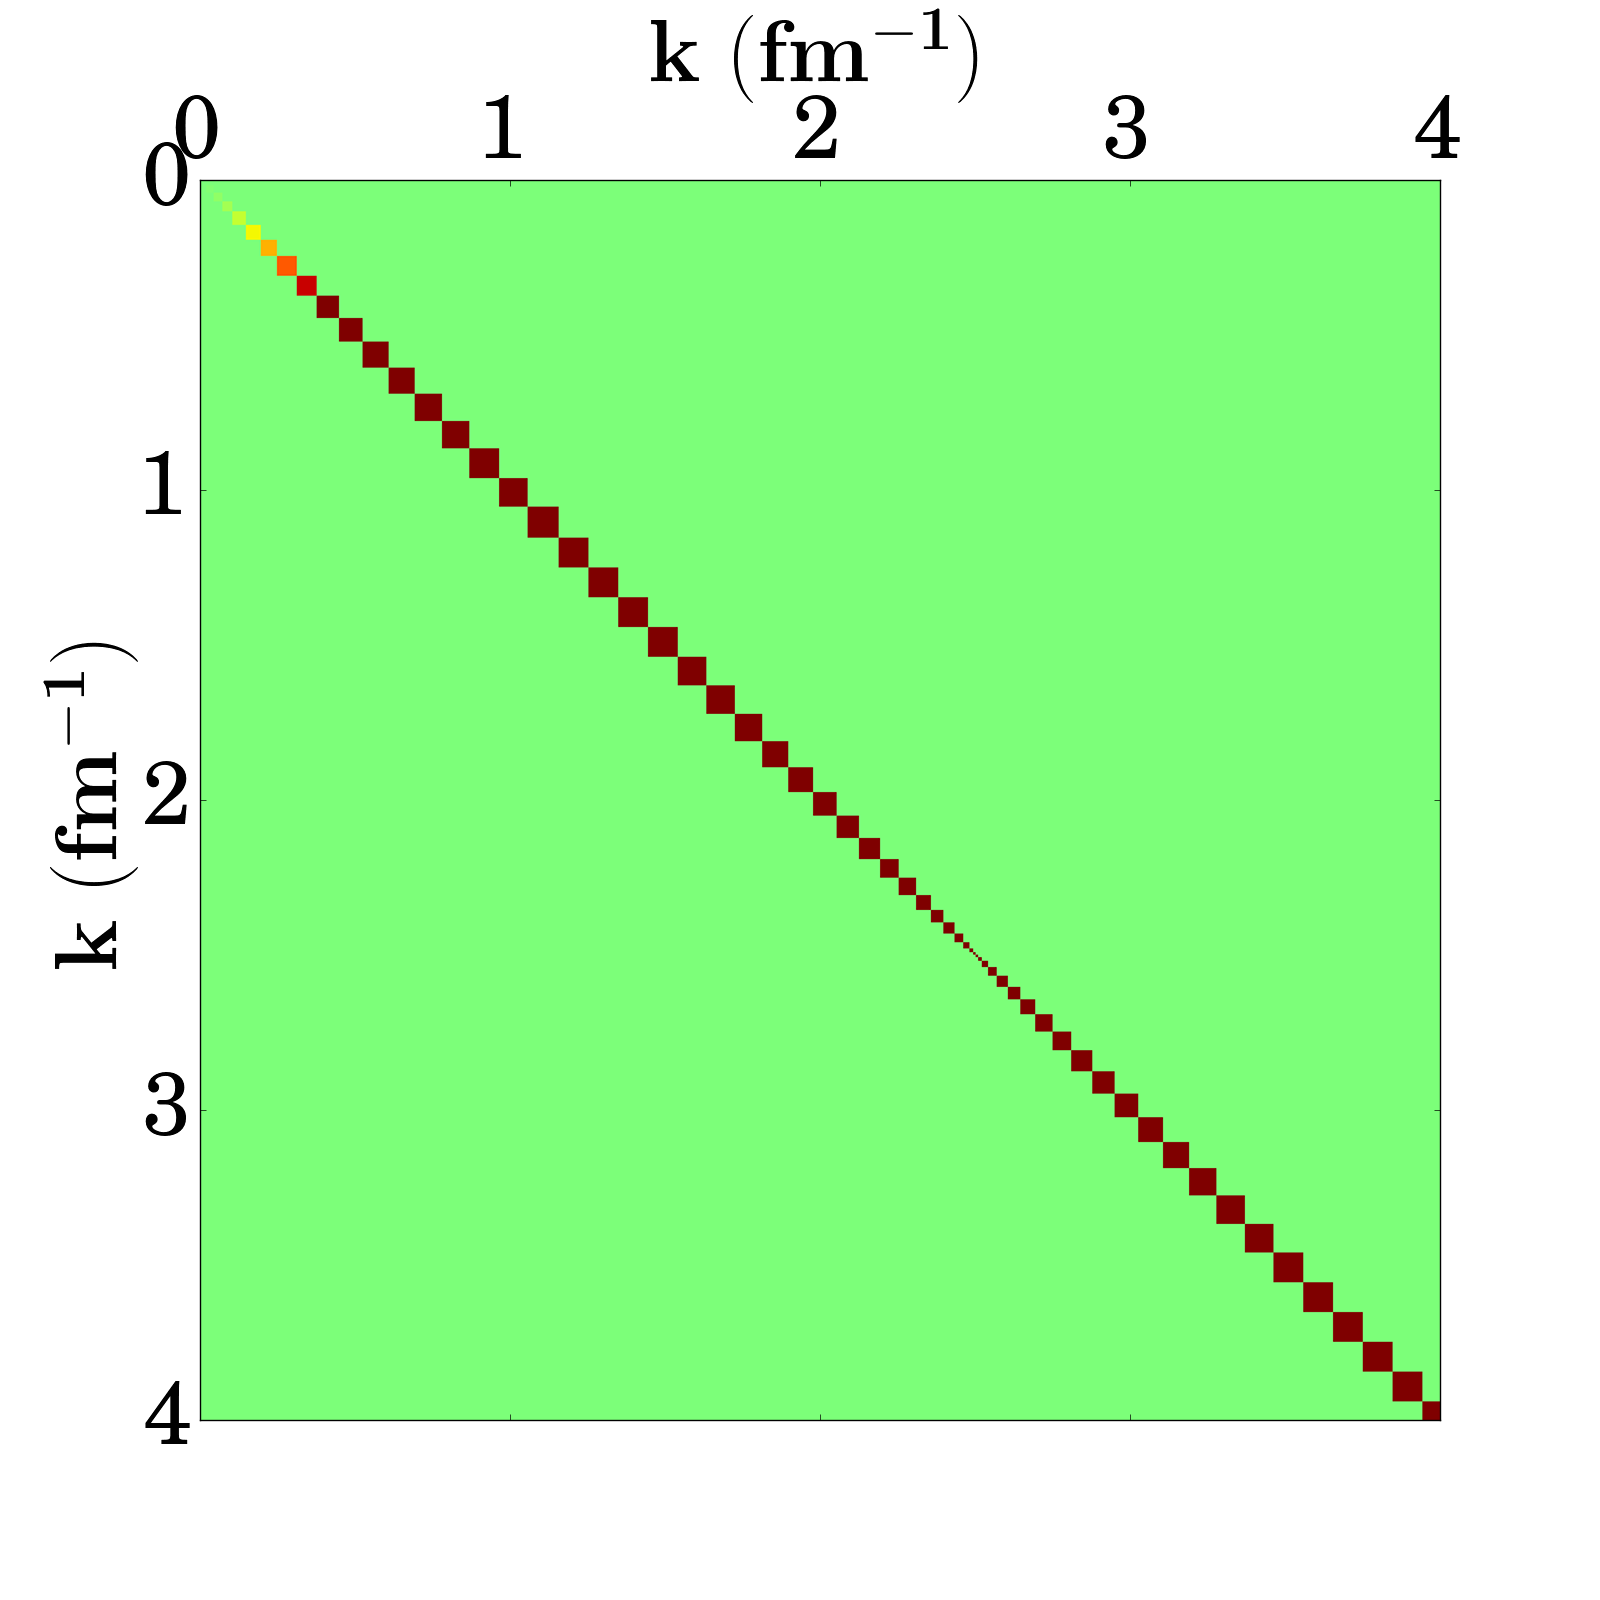
\includegraphics[trim={0 3cm 0 0},clip,width=0.25\linewidth]{T_generator}}
\subfloat[Evolution of $\hat{V}_s$\label{fig:2body_T_ev}]{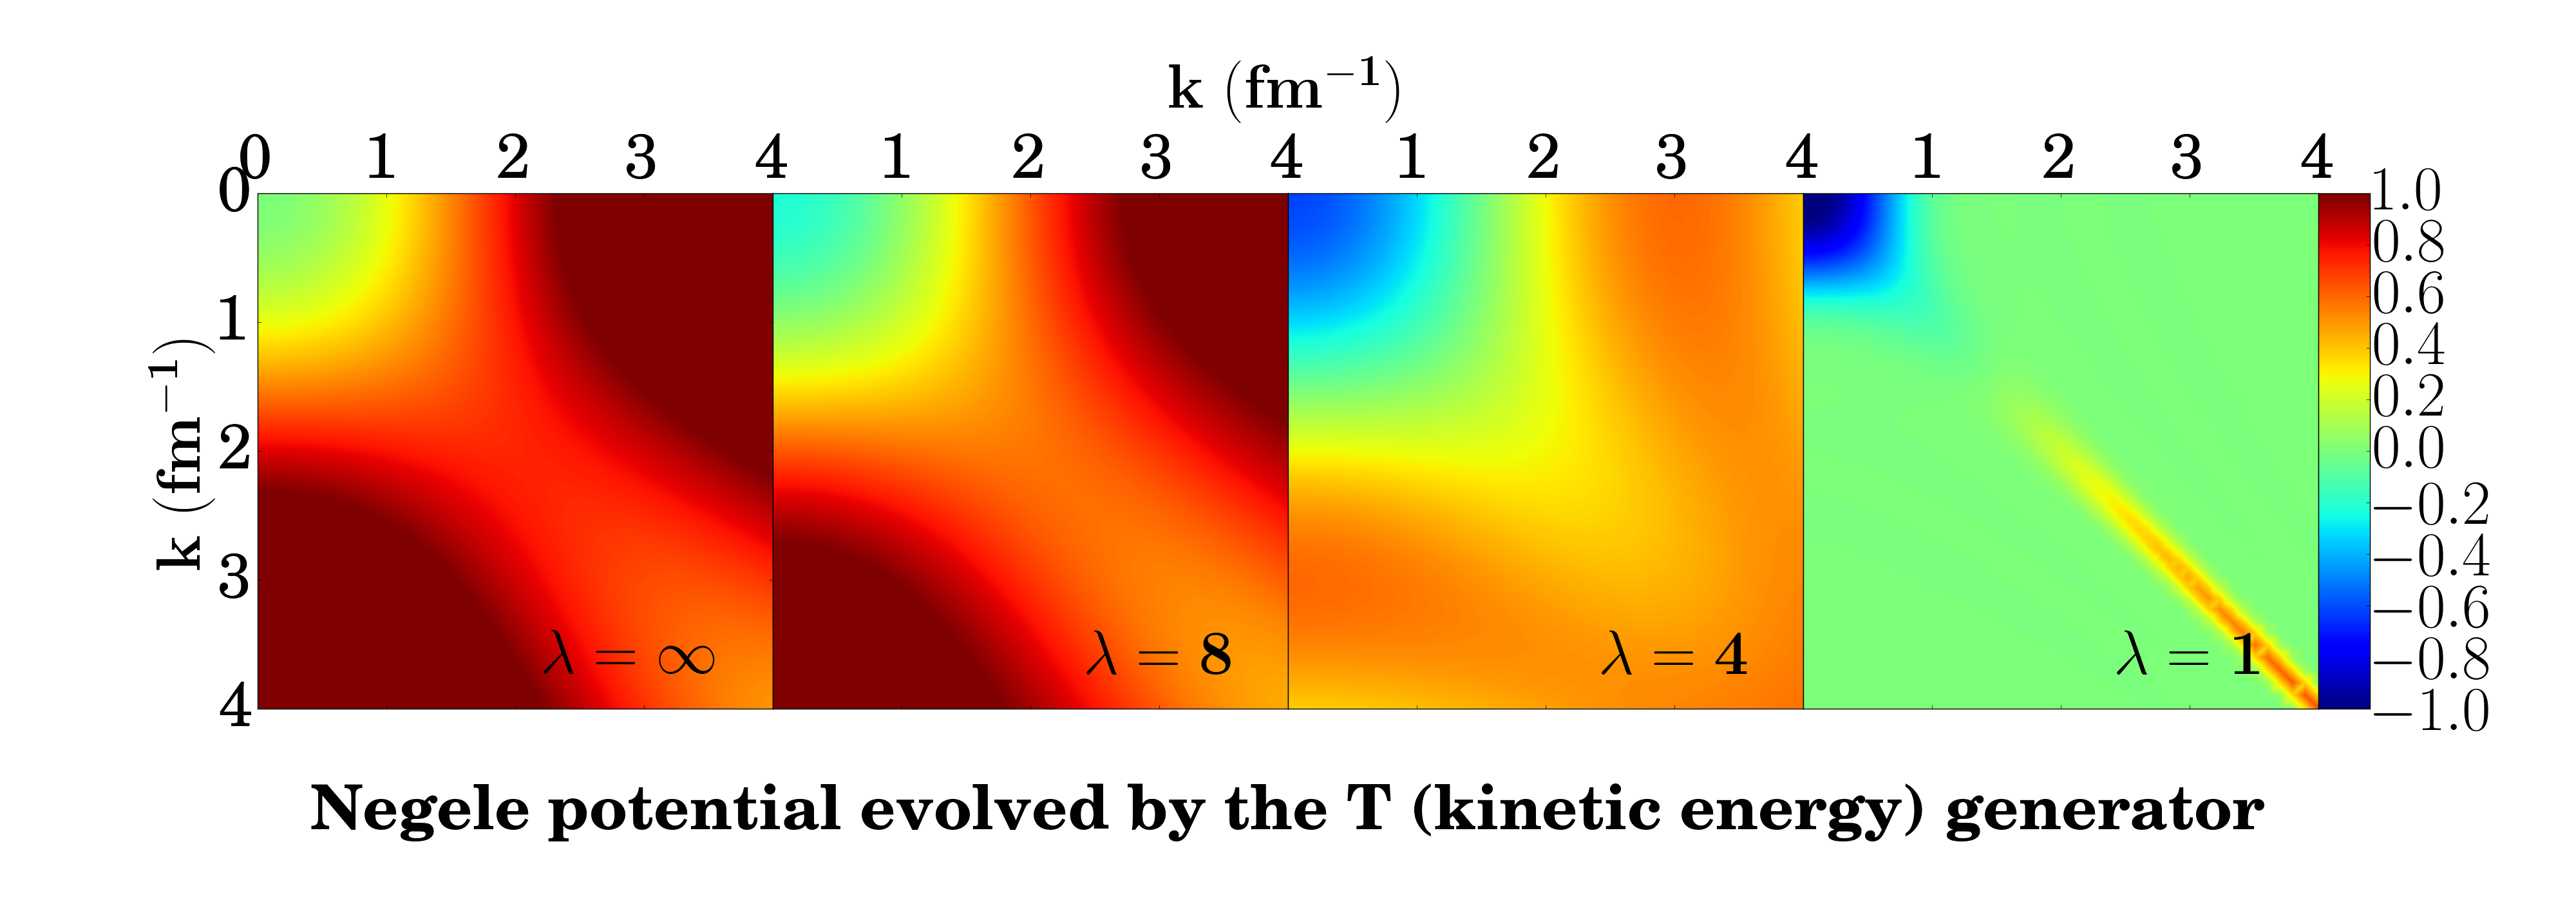
\includegraphics[trim={0 5cm 0 0},clip,width=0.75\linewidth]{T_evolution}}
\end{center}
\caption{Evolution from $\lambda=\infty$ to $\lambda=1$ of the even part of the $\hat{V}_\alpha$ potential in 2-body momentum space with $\hat{G}_s=\hat{T}$ as shown in (a).}
\label{fig:2body_T_full}
\end{figure}

\begin{figure}[th!]
\begin{center}
\subfloat[$\hat{G}_s=\hat{H}_{BD, s=0}$\label{fig:2body_BD_gen}]{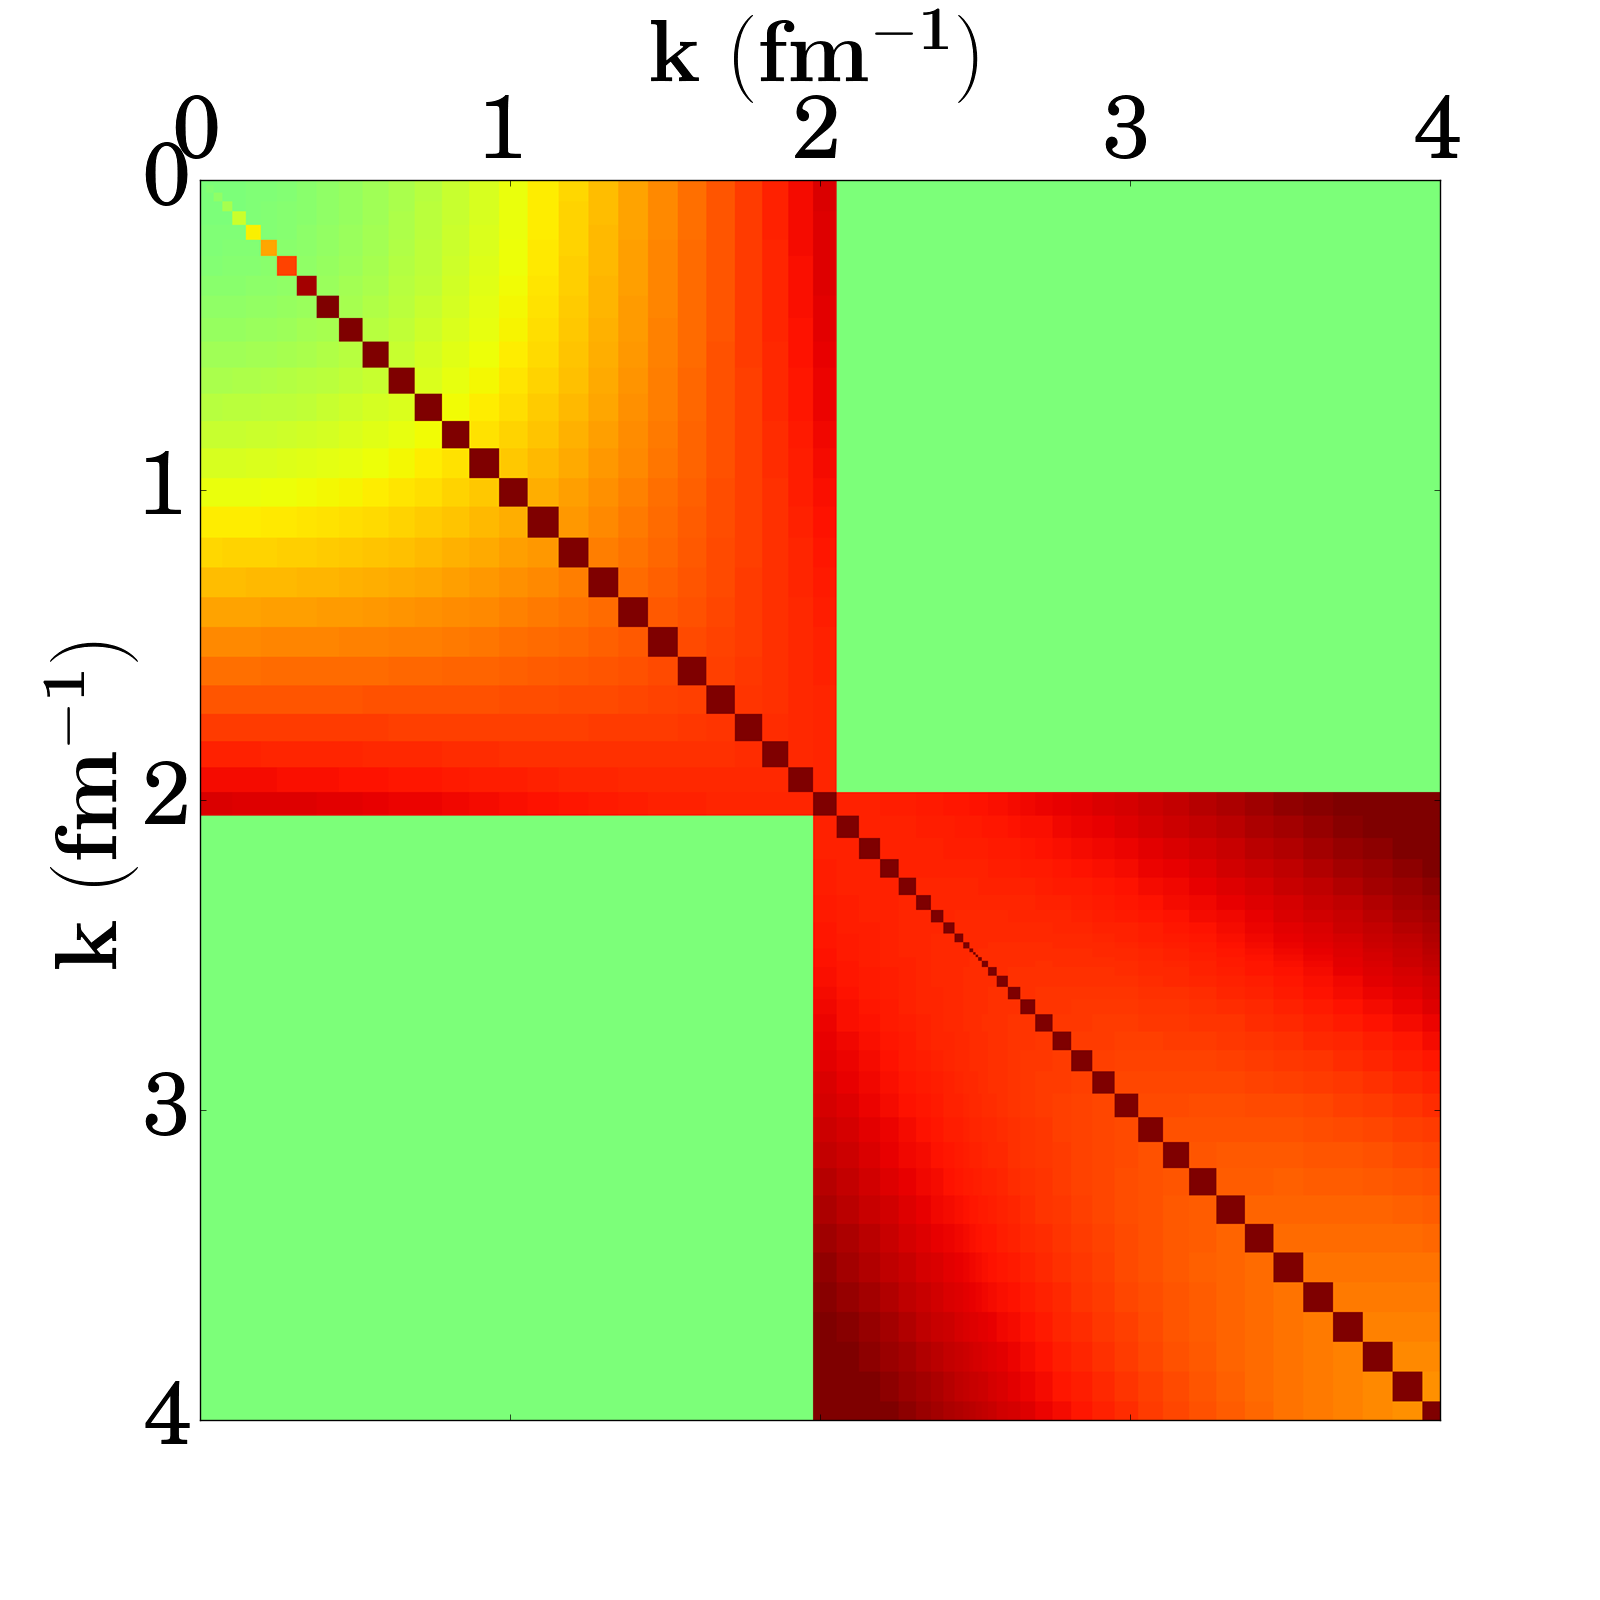
\includegraphics[trim={0 3cm 0 0},clip,width=0.25\linewidth]{BD_1_generator}}
\subfloat[Evolution of $\hat{V}_s$\label{fig:2body_BD_ev}]{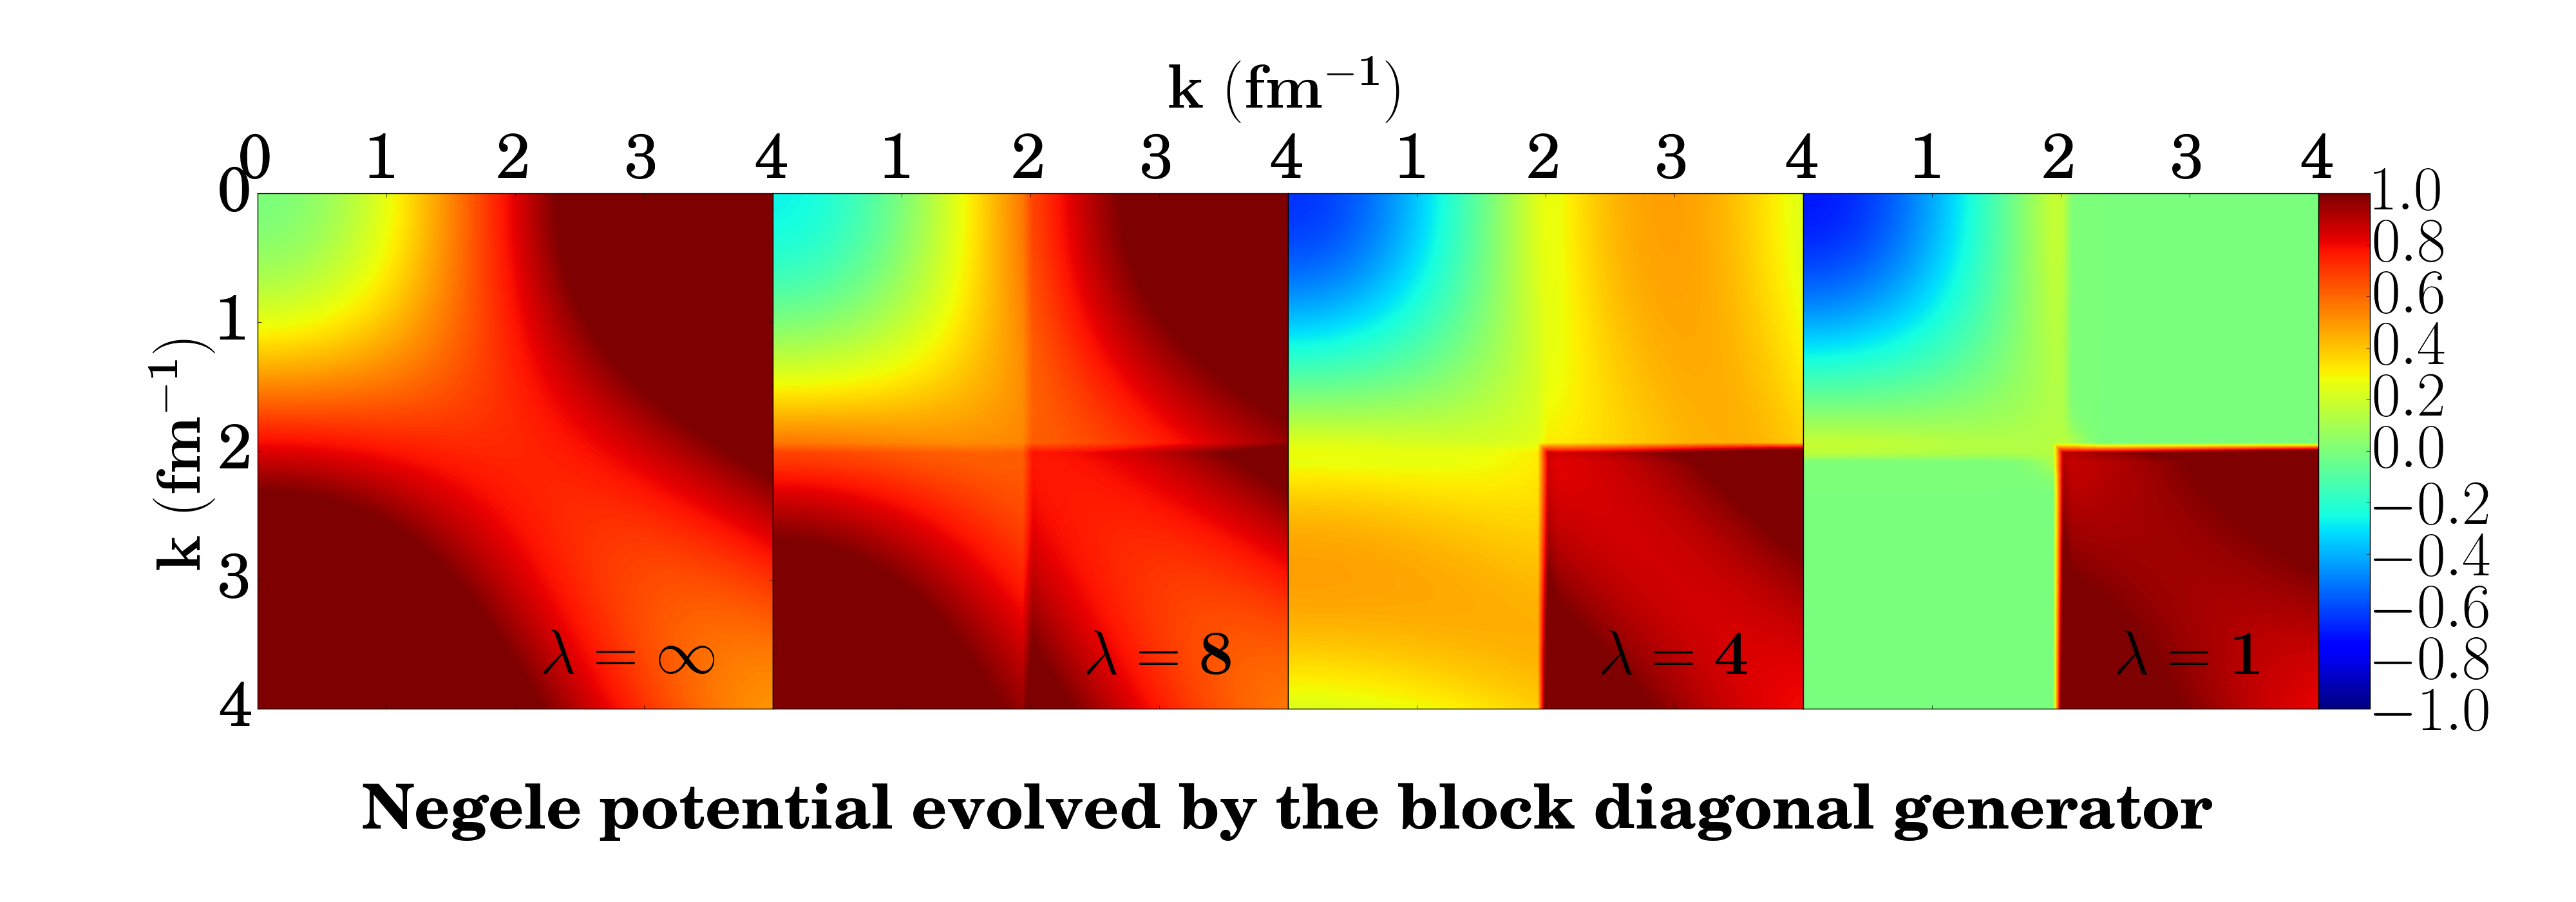
\includegraphics[trim={0 5cm 0 0},clip,width=0.75\linewidth]{BD_1_evolution}}
\end{center}
\caption{Evolution from $\lambda=\infty$ to $\lambda=1$ of the even part of the $\hat{V}_\alpha$ potential in 2-body momentum space with $\hat{G}_s=\hat{H}_{BD, s}$ as shown in (a).}
\label{fig:2body_BD_full}
\end{figure}

In computing the 2-body Hamiltonian from the Negele potential, we find the 2-body ground state energies to be $-0.920$ for $\hat{V}_\alpha$ and $-0.474$ for $\hat{V}_\beta$, consistent with previous results. Furthermore, the SRG evolution with $\hat{G}_s=\hat{T}$ of $\hat{V}_\alpha$ shown in Fig.~\ref{fig:2body_T_full} matches Fig.~\ref{fig:jurg_2body_ev}. The ground state energy eigenvalues are also preserved up to the error in the numerical solver used, confirming that the SRG method for a 2-body operator in a 2-body basis is unitary. In Fig.~\ref{fig:2body_BD_full}, we show the SRG evolution using a different flow operator, a block diagonal matrix with two blocks defined as
\begin{equation}\label{eq:H_bd_p}
\hat{G}_s = \hat{H}_{BD} = \hat{T} + \hat{V}_s \Theta(p - \Lambda) \Theta(p' - \Lambda) + \hat{V}_s \Theta(\Lambda - p) \Theta(\Lambda - p'),
\end{equation}
where $\Lambda$ is the cutoff momentum that defines the two blocks. For our purposes, we used $\Lambda=2 fm^{-1}$. The value of $\hat{H}_{BD}$ at $\lambda=\infty$ is shown in Fig.~\ref{fig:2body_BD_gen}.

The results of the SRG evolution with this flow operator are shown in Fig.~\ref{fig:2body_BD_ev}. This offers a good way to visualize how alternative generators change the form to which the SRG method evolves operators. The reason for applying SRG to an operator is to reduce the basis size required to accurately preserve low-energy eigenvalues. What this means is that we want the coupling between the low-energy sector we want to keep and the high-energy sector we want to discard to be zero. Applying SRG with $\hat{G}_s=\hat{T}$ does more than this, driving the entire operator toward the diagonal, even in the low-energy block. It is important to note that if all the low-energy physics is contained inside the low-energy block, we do not care if the matrix is diagonal or not in that block; we have already successfully reduced the size of the problem. Alternative flow operators can be chosen to better reflect these goals, and the intuition is that by avoiding doing unnecessary decoupling, SRG with these flow operators may induce smaller many-body forces. We want to put this intuition to the test when we reach the 3-body case.

% The reason for exploring such generators is that SRG with $\hat{G}_s=\hat{T}$ essentially fully diagonalizes the Hamiltonian. SRG with alternative generators that do not force decoupling of slightly off-diagonal elements may do less ``work" and therefore induce fewer many-body forces. We want to put this intuition to the test when we reach the 3-body case.

\subsection{Harmonic Oscillator Space Transformation}
\begin{figure}[t]
\begin{center}
\subfloat[$\hat{V}_\alpha$\label{fig:2body_a_nmax}]{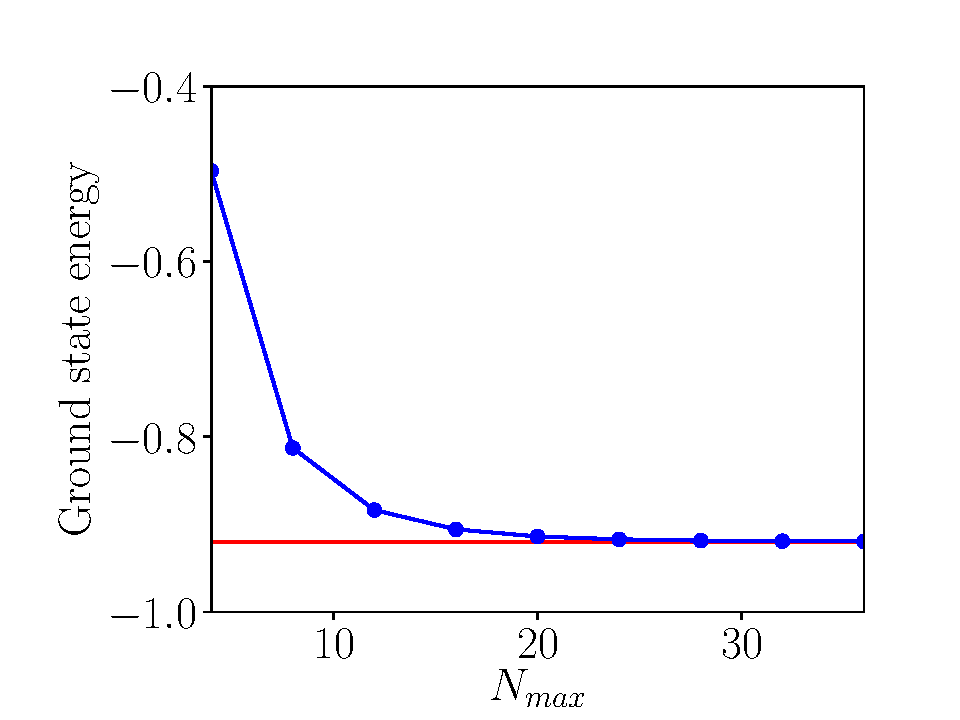
\includegraphics[width=0.5\linewidth]{alpha_2body_nmax}}
\subfloat[$\hat{V}_\beta$\label{fig:2body_b_nmax}]{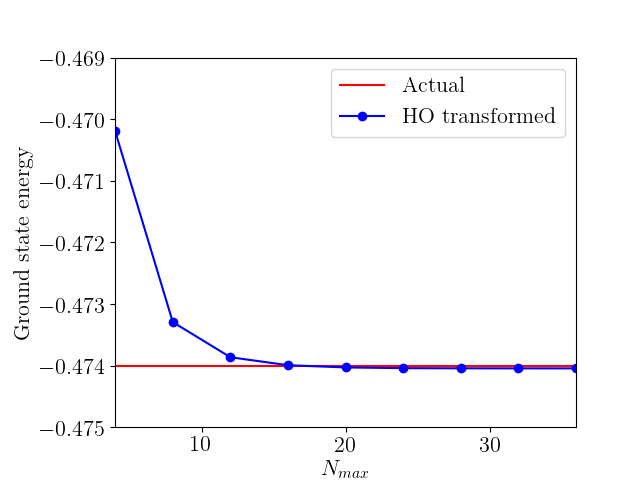
\includegraphics[width=0.5\linewidth]{beta_2body_nmax}}
\end{center}
\caption{2-body harmonic oscillator basis convergence patterns for (a) $\hat{V}_\alpha$ and (b) $\hat{V}_\beta$ with respect to $N_{max}$.}
\label{fig:2body_nmax}
\end{figure}

To lay the groundwork for exploring the 3-body system, we transform our 2-body operators into a symmetric harmonic oscillator basis. In practice, we truncate our harmonic oscillator basis at some maximum total harmonic oscillator number, $N_{max}$. We use $N_{max}=28$, and we show in Fig.~\ref{fig:2body_nmax} that by this value the 2-body ground state eigenvalue is converged to the value calculated in momentum space to within 0.1\%.

\begin{figure}[t]
\begin{center}
\subfloat[$\hat{T}$ transformed\label{fig:kin_e_transformed}]{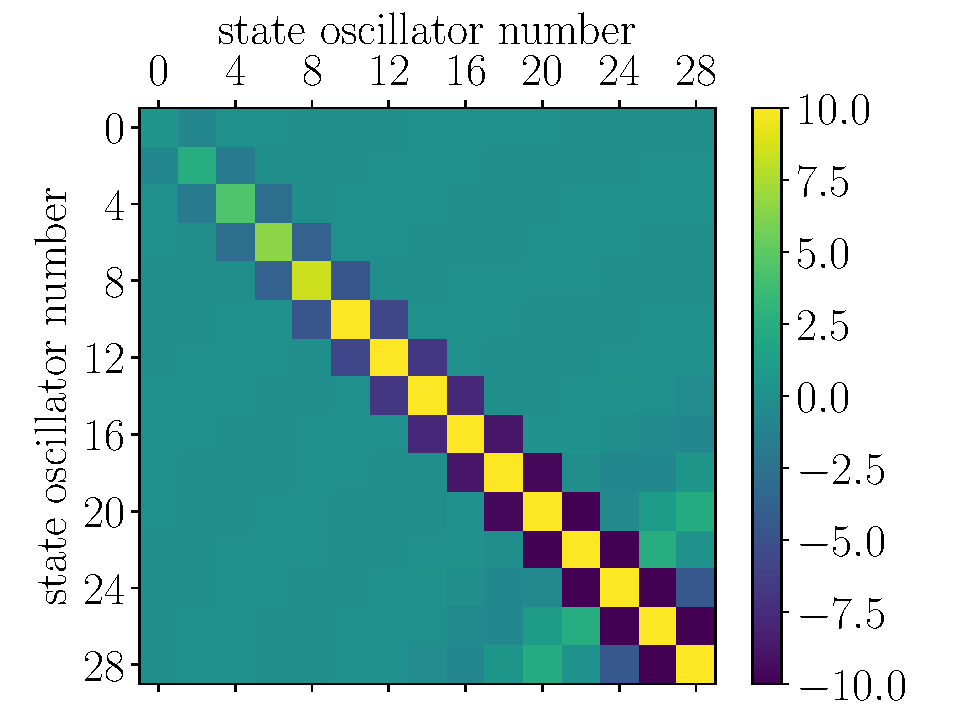
\includegraphics[trim={0 0 4cm 0},clip,width=0.43\linewidth]{transform_kin_e}}
\subfloat[$\hat{T}$ from HO basis\label{fig:kin_e_ho}]{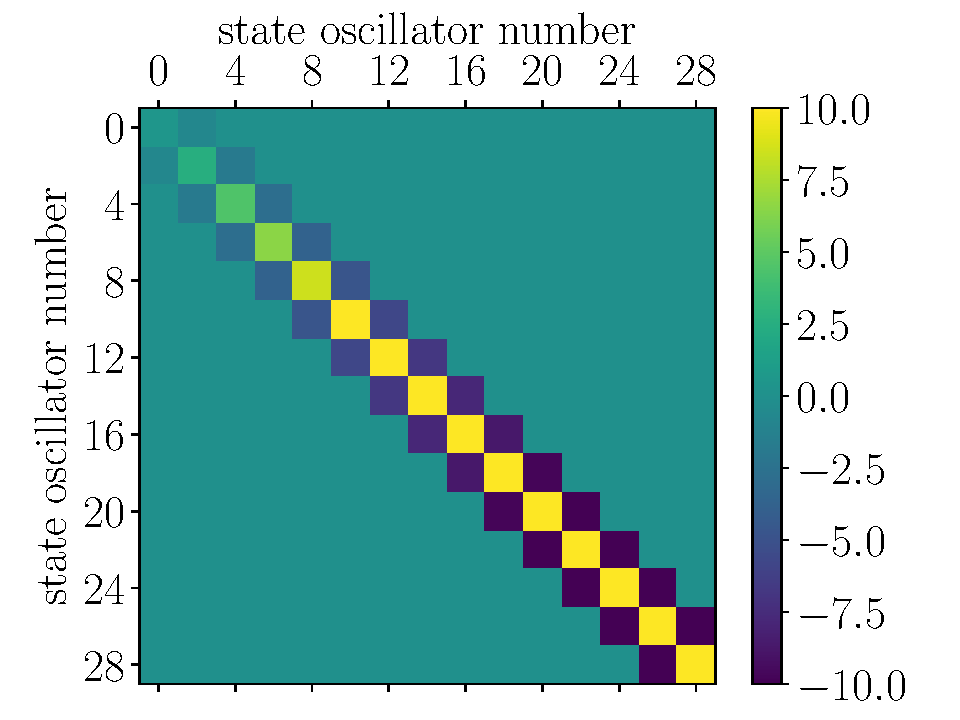
\includegraphics[trim={0 0cm 0 0},clip,width=0.57\linewidth]{pure_kin_e}}
\end{center}
\caption{The harmonic oscillator kinetic energy operator as computed (a) via a transformation from the momentum space operator and (b) directly from the harmonic oscillator basis.}
\label{fig:2body_kin_comp}
\end{figure}

As an additional check, we compare the kinetic energy calculated in momentum space and transformed to harmonic oscillator space to the kinetic energy operator computed directly from the symmetric harmonic oscillator basis. We find in Fig.~\ref{fig:2body_kin_comp} that they are the same at low harmonic oscillator number, which corresponds to low energies. At high energies, we see the transform kinetic energy operator stray from the true tridiagonal form of the kinetic energy in harmonic oscillator space. This is caused by ringing due to the truncation of the harmonic oscillator basis. However, this ringing does not affect the low-energy parts of the kinetic energy and thus has no effect on the lowest eigenvalues, the bound state energies we care about preserving. For the 3-body case we will be working with the transformed potential energy and the kinetic energy computed directly from the harmonic oscillator basis, as it is cleaner to calculate and does not have the ringing artifacts.%At high energies, we see the transform kinetic energy operator stray from the true tridiagonal form of the kinetic energy in harmonic oscillator space. This is caused by ringing due to the truncation of the harmonic oscillator basis. However, this ringing does not affect the low-energy parts of the kinetic energy and thus has no effect on the lowest eigenvalues, the bound state energies we care about preserving. 

\section{3-Body}

\begin{figure}[t]
\begin{center}
\subfloat[$\hat{V}_\alpha$\label{fig:3body_a_nmax}]{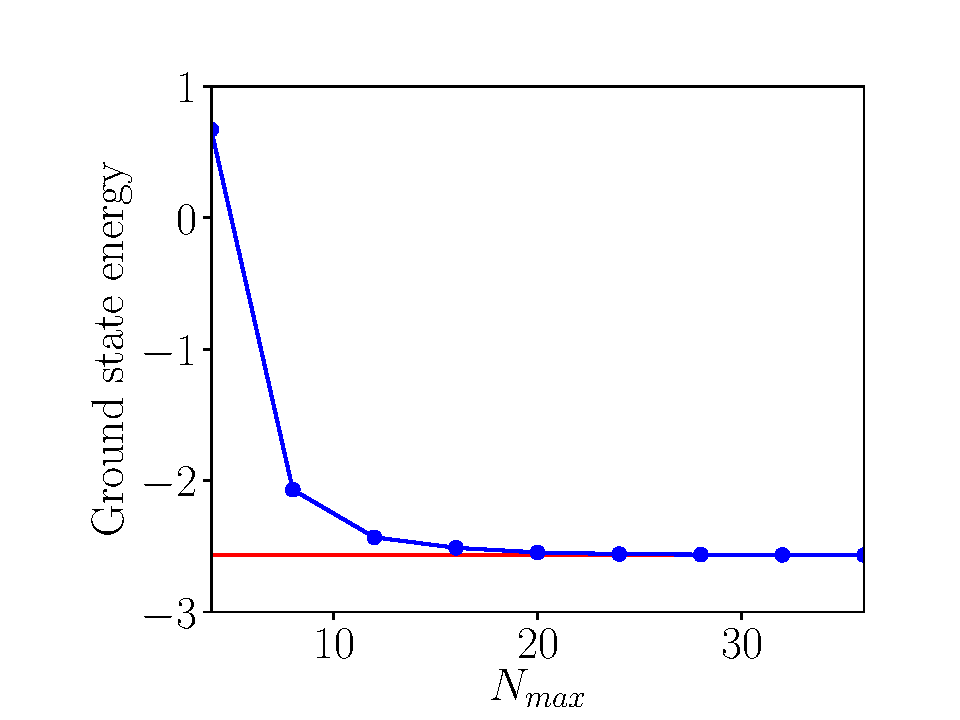
\includegraphics[width=0.5\linewidth]{alpha_3body_nmax}}
\subfloat[$\hat{V}_\beta$\label{fig:3body_b_nmax}]{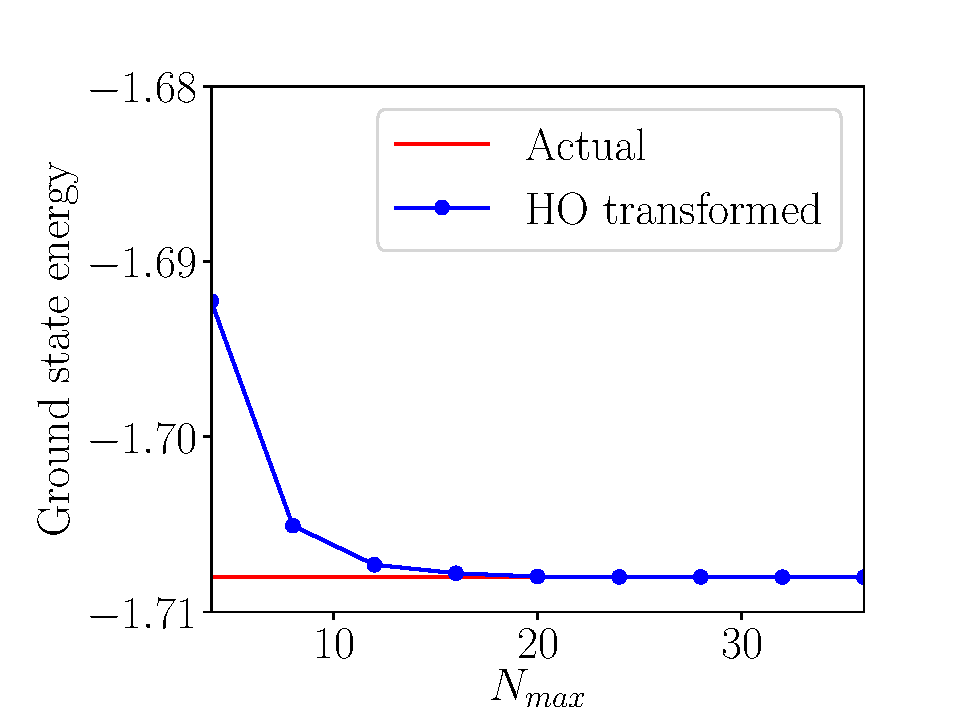
\includegraphics[width=0.5\linewidth]{beta_3body_nmax}}
\end{center}
\caption{3-body harmonic oscillator basis convergence patterns for (a) $\hat{V}_\alpha$ and (b) $\hat{V}_\beta$ with respect to $N_{max}$.}
\label{fig:3body_nmax}
\end{figure}

For the 3-body system, the key results for us to reproduce are the 3-body ground state energies in Table \ref{table:negele_params} and the induced 3-body force in Fig.~\ref{fig:jurg_vfull} for $\hat{G}_s=\hat{T}$.

\subsection{3-Particle Ground State}

For the 3-body symmetric harmonic oscillator basis, we stay with $N_{max}=28$ in order to replicate the same results as Ref.~\cite{Jurgenson:2008jp}. There is also a performance consideration here, because, while the basis size for a 2-body system scales linearly in $N_{max}$, the basis size for a 3-body system scales quadratically in $N_{max}$. Since at $N_{max}=28$ we are already converged to within 1\% in the 3-body system, as shown in Fig.~\ref{fig:3body_nmax}, by raising $N_{max}$ we would simply be slowing down our ability to test alternative flow generators without any substantial numerical gain. With $N_{max}=28$, we get the 3-body ground state energy to be $-2.563$ for $\hat{V}_\alpha$ and $-1.708$ for $\hat{V}_\beta$, matching the values listed in Table \ref{table:negele_params}.

\begin{figure}[t]
\begin{center}
\subfloat[2-body ground state energy\label{fig:2body_a_w}]{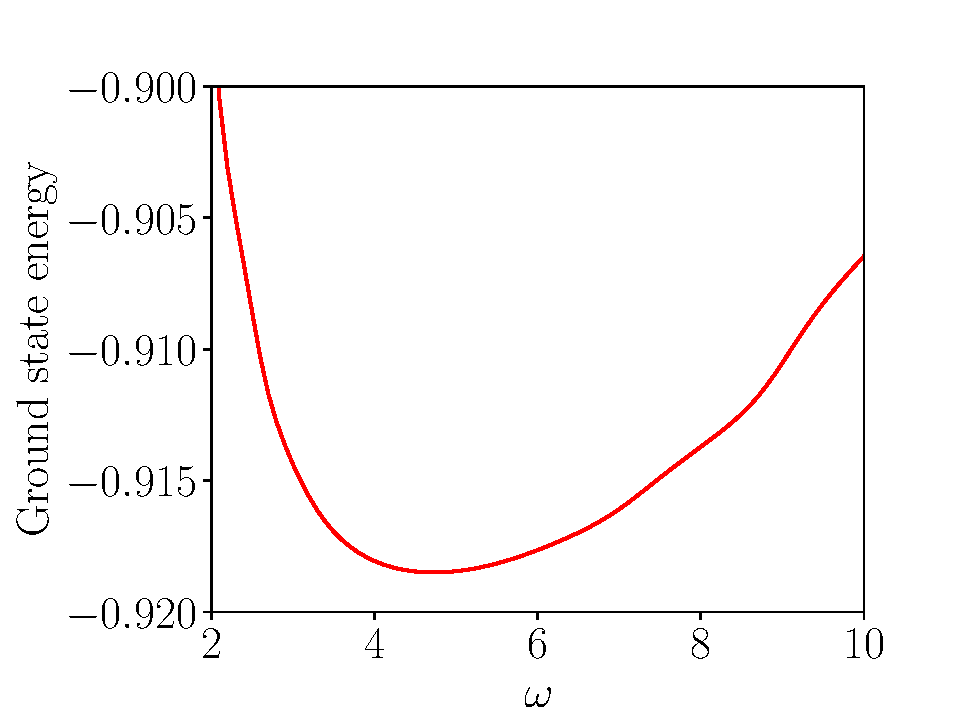
\includegraphics[width=0.5\linewidth]{alpha_2body_w}}
\subfloat[3-body ground state energy\label{fig:3body_a_w}]{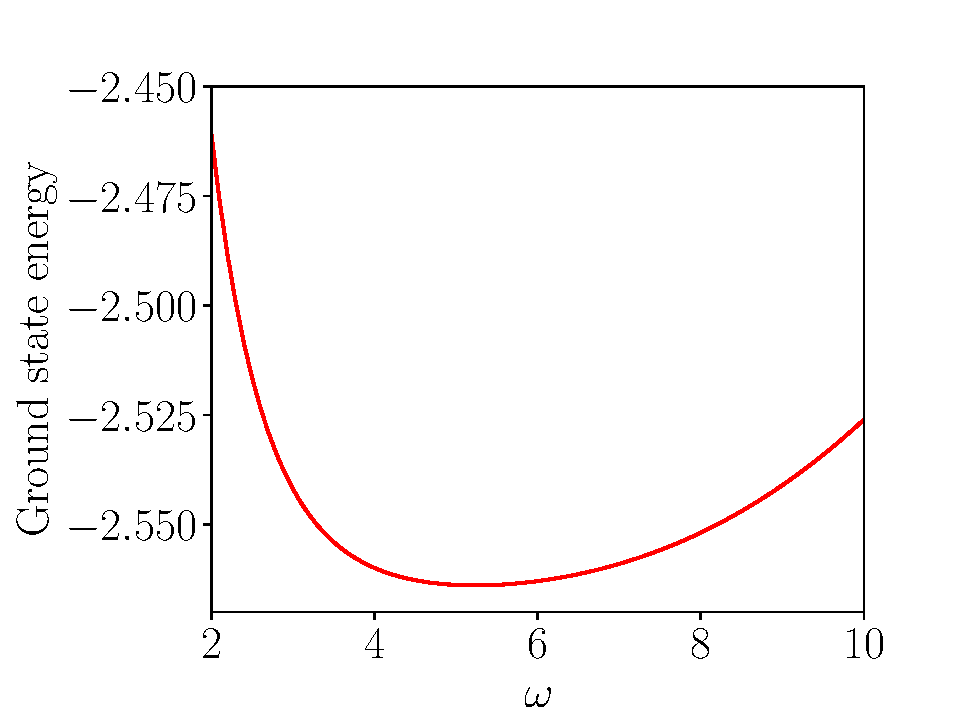
\includegraphics[width=0.5\linewidth]{alpha_3body_w}}
\end{center}
\caption{Ground state energy is a smooth function of $\omega$ and thus easy to minimize.}
\label{fig:alpha_w}
\end{figure}

When going from momentum space to harmonic oscillator space, we must optimize $\omega$, the parameter for the harmonic oscillator basis. The optimal $\omega$ will minimize the ground state energy, which will be the best we can do to reproduce the low-energy eigenvalues for a given $N_{max}$. We find that roughly the same value for $\omega$ optimizes both the 2-body ground state energy and the 3-body ground state energy, as shown in Fig.~\ref{fig:alpha_w}.


\subsection{3-Body Force Induction for $\hat{G}_s=\hat{T}$}

We then compare the 3-body ground state values for a Hamiltonian evolved in 3-body systems and a Hamiltonian evolved in the 2-body system and embedded in the 3-body system at each intermediate point during the evolution. We see in Fig.~\ref{fig:heinz_vfull} the same trends as in Fig.~\ref{fig:jurg_vfull}. With this, we have verified the correctness of our framework up to the 3-body system and can now use it to test the 3-body force induction of SRG with alternative flow operators.

\begin{figure}[t]
\begin{center}
\subfloat[$\hat{V}_\alpha$\label{fig:heinz_va}]{\centering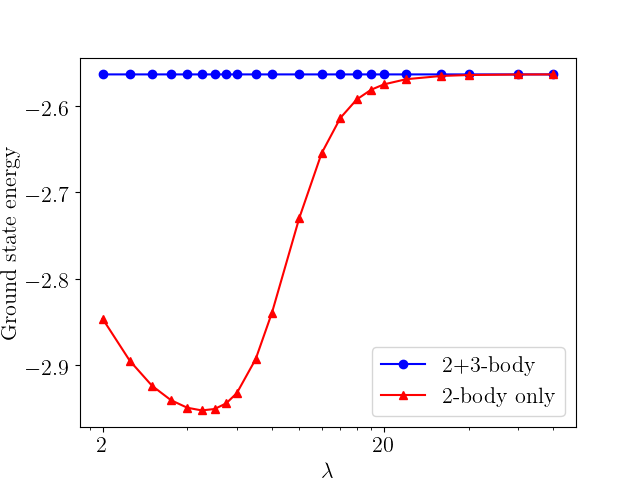
\includegraphics[width=0.5\linewidth]{manybody_T_alpha}}
\subfloat[$\hat{V}_\beta$\label{fig:heinz_vb}]{\centering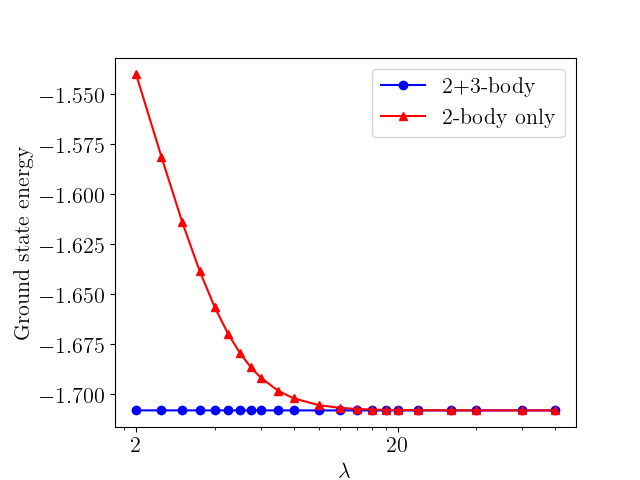
\includegraphics[width=0.5\linewidth]{manybody_T_beta}}
\end{center}
\caption{3-body force induction with $\hat{G}_s=\hat{T}$ leading to error in the computed 3-body ground state energy.}
\label{fig:heinz_vfull}
\end{figure}

\subsection{3-Body Force Induction for Alternative Flow Operators}

We test two parametrizations for an alternative flow operator, $\hat{H}_{BDHO}$, that is block diagonal in harmonic oscillator space, defined as
\begin{equation}
\hat{G}_s = \hat{H}_{BDHO} = \hat{T} + \hat{V} \Theta(N - \Lambda) \Theta(N' - \Lambda),
\end{equation}
where $\Lambda$ is the block cutoff in harmonic oscillator space. We use $\Lambda=6$ and $\Lambda=10$ for our tests. We find that both parametrizations offer a substantial decrease in the induced 3-body force, as shown in Fig.~\ref{fig:heinz_newfull}. In particular, $\Lambda=10$ induces nearly no 3-body force, keeping the 3-body ground state energy within less than 1\% of its true value.

\begin{figure}[th!]
\begin{center}
\subfloat[$\hat{V}_\alpha$\label{fig:heinz_newa}]{\centering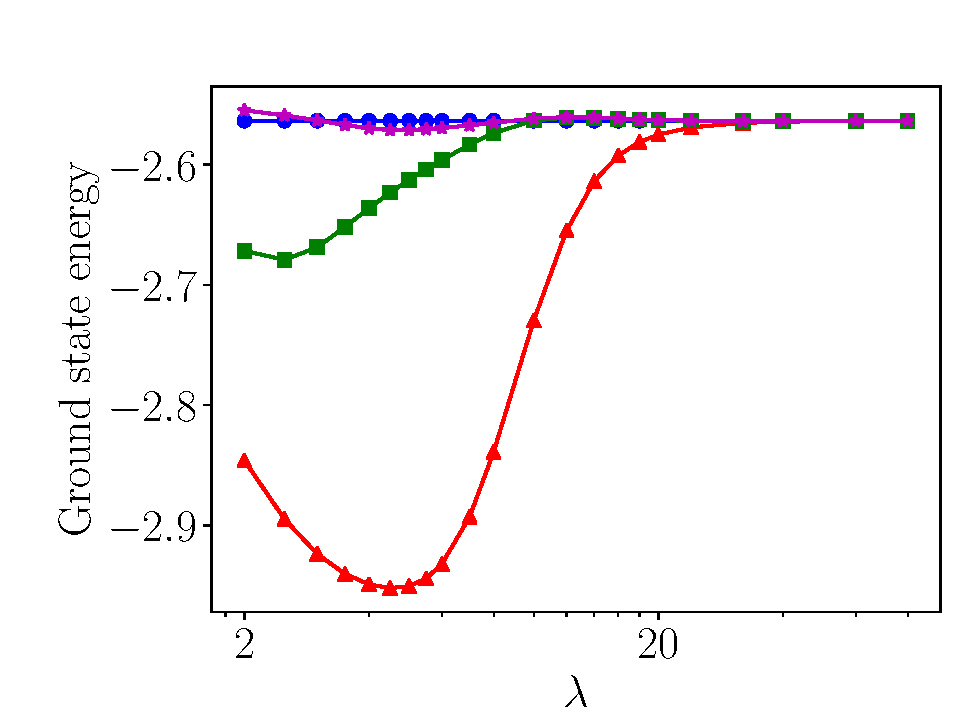
\includegraphics[width=0.5\linewidth]{new_alpha}}
\subfloat[$\hat{V}_\beta$\label{fig:heinz_newb}]{\centering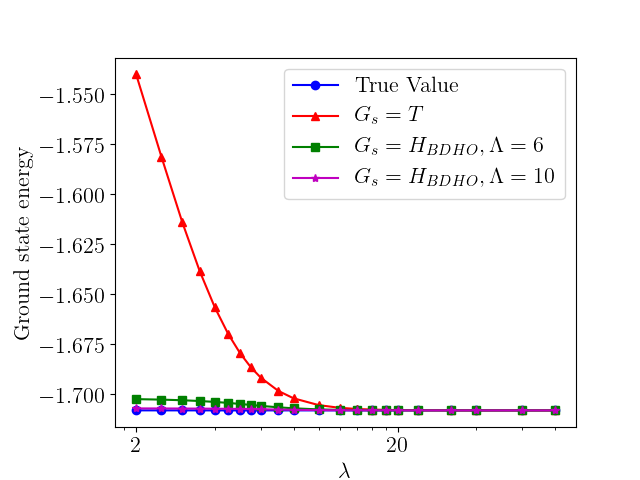
\includegraphics[width=0.5\linewidth]{new_beta}}
\end{center}
\caption{3-body force induction for various different generators. We see $\hat{H}_{BDHO}$ leads to a generally smaller induced 3-body force.}
\label{fig:heinz_newfull}
\end{figure}

While these results show promise for $\hat{H}_{BDHO}$ as an improved flow operator, they are still preliminary. It may be the case case that $\hat{H}_{BDHO}$ and $\hat{T}$ decouple off-diagonal matrix elements at different rates with respect to $\lambda$, meaning that $\lambda=1$ for $\hat{T}$ evolutions does not correspond to $\lambda=1$ for $\hat{H}_{BDHO}$ evolutions. While some quick tests ``by eye" suggest this is not the case, it must still be verified more robustly. This can be done by imposing some cutoff on the 2-body space and checking that the $\lambda$ at which both evolutions reproduce the correct ground state energy is similar. If it is not similar, it will be necessary to figure out a mapping of corresponding values of $\lambda$ for the two evolutions.

Additionally, tests must be run that look at 4-body and 5-body forces, in order to ensure induced many-body forces remain strictly smaller than for $\hat{G}_s=\hat{T}$. The \texttt{srg1d} framework also allows us to easily test more flow operators, which we must do to get a more comprehensive idea of what features of the flow operators reduce or enhance many-body force induction.


